
% INSTRUCTIONS:
% To compile this file, run "latex HW_example";  you need to do it TWICE
%    to get the cross-references (to equations, etc) to show correctly.
% Figures can be included as shown below.  If you don't have a figure,
%    comment out those lines using % signs at the beginning of each line,
%    or else just keep hitting RETURN when LaTeX gives an error message
%    saying that it can't find the figure file.
% Run "dvips HW_example.dvi" to make a Postscript file HW_example.ps,
%    and then "ps2pdf HW_example.ps" to make a PDF file HW_example.pdf.

\documentclass[12pt]{article}
\usepackage{graphicx,indentfirst}

\pagestyle{plain}
\baselineskip 18pt
\textwidth 6.5in
\textheight 7.8in
\oddsidemargin 0.1in
\evensidemargin 0.1in
\topmargin 0.3in

\newcommand{\be}{\begin{equation}}
\newcommand{\ee}{\end{equation}}
\newcommand{\reff}[1]{(\ref{#1})}


\begin{document}

\title{Computational Physics \\ Homework 6}
\author{Yi-Hsuan Hsu}
\date{11/18/2014}
\maketitle

\section{Problem}
Solve 2-dimension Poisson equation with periodic boundary condition by multi-grid Gauss Seidel algorithm. Using block average and piecewise-constant injection for restriction and prolongation. Measuring and comparing asymptotic convergence rate of V-circle and W-circle. In question (d), investigating the effect of pre- and post sweeps. In question (e), Over-relaxation Gauss Seidel should be integrated. Find out the optimized parameter for convergence rate. In question (f), instead of piecewise-constant, using nine-point restriction and prolongation method and discussing and result. In the exercise, I will use periodic testing function as below
\begin{eqnarray}
		&&\triangle^2 \phi=f(x,y)\nonumber\\
		&&\phi=sin(2\pi x)sin(2\pi y)\nonumber\\
		&& f(x,y)=-8\pi^2sin(2\pi x)sin(2 \pi y)
\end{eqnarray}

\subsection{Algorithms}

Overralaxation$(SOR)$ Guass Seidel method from previous lecture are continuing using as core iteration method.
\begin{eqnarray}
v_{m_1,i,j}&=&(1-w)v_{m,i,j}+ w(v_{m,i-1}+v_{m,i+1,j}+v_{m,i,j-1}+v_{m,i,j+1}+h^2f_{ij})/4\\
v_{m_1,i,j}&=&(1-w)v_{m+1,i,j}+w(v_{m+1,i-1}+v_{m+1,i+1,j}+v_{m+1,i,j-1}+v_{m+1,i,j+1}+h^2f_{ij})/4
\end{eqnarray}

However, the convergence of Gauss Seidel method depends on grid number $N$. The reason is that GS method take average of neighboring grid to calculate new approximation in each iteration. Therefore, information propagates only one grid in every single step. More, one can prove that it would take at least $O(log(N)$ steps to decreasing the error by the factor of one.

\begin{figure}[h!]
	\begin{center}
		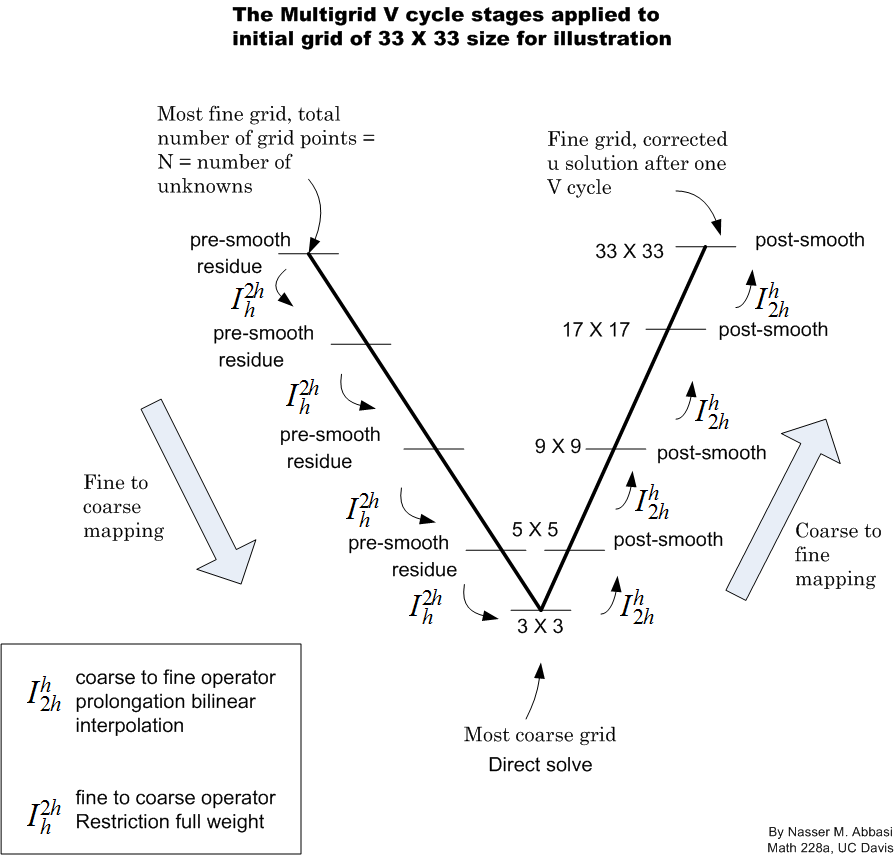
\includegraphics[width=0.5\textwidth]{multigrid_V.png}
		\caption{V-circle multi-grid method reduce the grid number half in each dimension. Pic. from $www.mgnet.org$}
		\label{fig1}
	\end{center}
\end{figure}

Multi-grid algorithm convert a N-by-N problem to a N/2-by-N/2 problem and reverse in order to accelerate information propagation. 

The restriction and prolongation operator transform fine grid to coarse grid. The piecewise-constant method restrict the grid by averaging four neighbor into one, and its adjoint prolongation copies the same value to its four neighbors. Fugure.2 shows an example of 4-by-4 matrix transformation.
\begin{figure}[h!]
	\begin{center}
		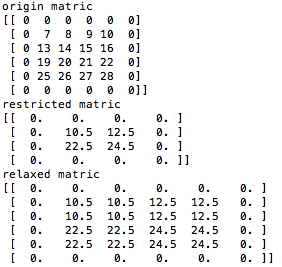
\includegraphics[width=0.5\textwidth]{restrict.png}
		\caption{Piecewise-constant restriction and relaxtion example}
		\label{fig2}
	\end{center}
\end{figure}
Smoothing iteration takes an approximate solution $\phi'$ to compute a better correction $\phi"=GS(\phi',f_1)$. Pre-smooth and Post-smooth can be the same of different. Note that iteration number in pre- and post-smoothing denoted by $(m_1,m_2)$. We may return to discuss the effect later.

In each stage, the right hand side $f$ is replaced by residual $r=A\phi'-f$, or in computer language
\begin{equation}
	r_{i,j}=-\frac{1}{N^2}(\phi'_{i-1,j}+\phi'_{i,j-1}\phi'_{i,j+1}\phi'_{i,j-1}-\phi'_{i,j})+f_{i,j}
\end{equation}

where $N$ is grid number in each coordinate.

V- or W- circle is controlled by parameter $\gamma$. V-circle ($\gamma$=1) smooths each stage one time. In the other hand, W-circle smooth $\gamma=2$ each stage two times. 


\subsection{Code description}
See comments in $src/multigridconst.py$
\subsection{Sample output}
\begin{figure}[h!]
	\begin{center}
		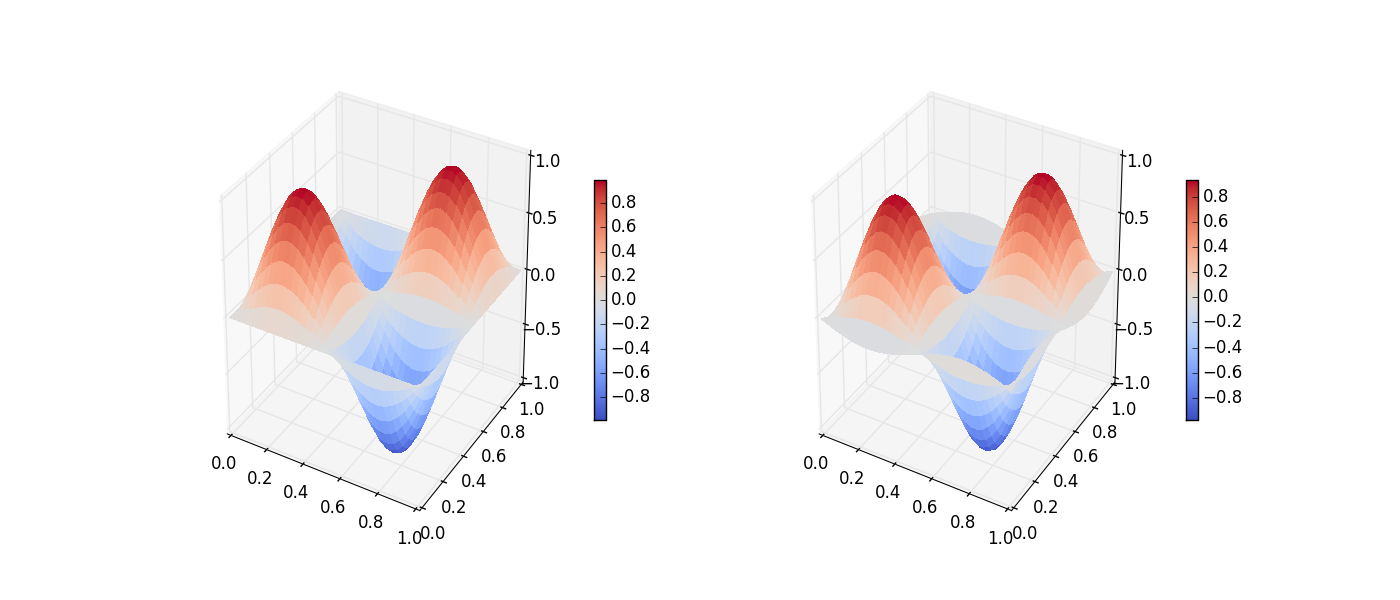
\includegraphics[width=0.8\textwidth]{Exact_Approx.png}
		\caption{RHS: Eaxcat solution. LHS:Approximation solution. Standard 5-point discretization, 25-by-25 in each coordination.}
		\label{fig3}
	\end{center}
\end{figure}
\subsubsection{Approximated solution}
Figure.3 shows approximation solution and exact solution using V-circle multi-grid algorithm. Offset error is setting by $\epsilon<10^{-8}$. The results show great approximation and convergence.

\subsubsection{Convergence rate as a function of lattice size}
Figure.4 illustrates the convergence rate by simple Gauss-Seidel, V-circle, W-circle method. The method of simple Gauss Seidel take six hundred circles0(6 steps per circle in order to comparison) to reach error offset, which is twenty times more than multi-grid method. The experiment proves that multi-grid method performs better than pure Gauss Seidel method. From the fitting line show in the picture we can conclude that V-circle converges slower than W-circle. Meanwhile, V-circle takes fewer time in computation due to W-circle conduct more computing in each circle.

Figure.5 demonstrates convergence rate as a function of Lattice size. Data shows a linear relation in between. In the other hand, computing time grows exponentially while lattice size goes up

\begin{figure}[h!]
	\begin{center}
		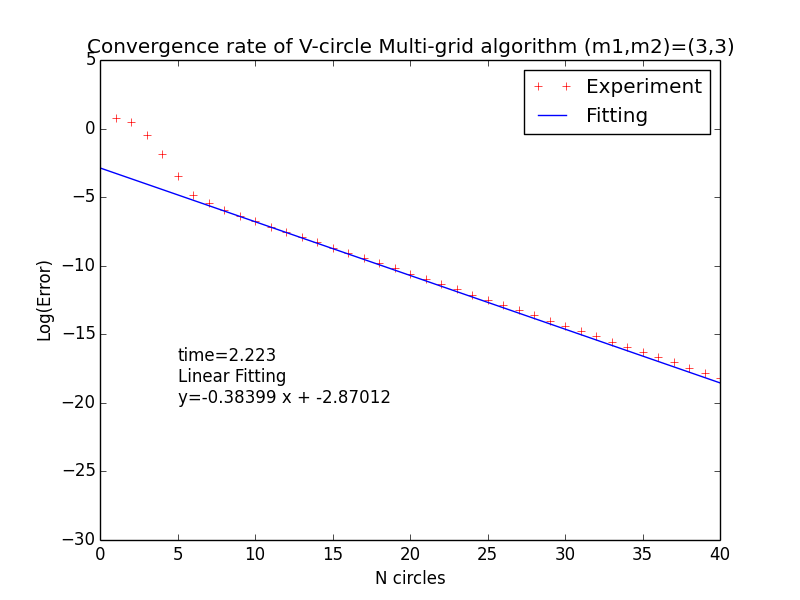
\includegraphics[width=0.4\textwidth]{V_converge_rate.png}
		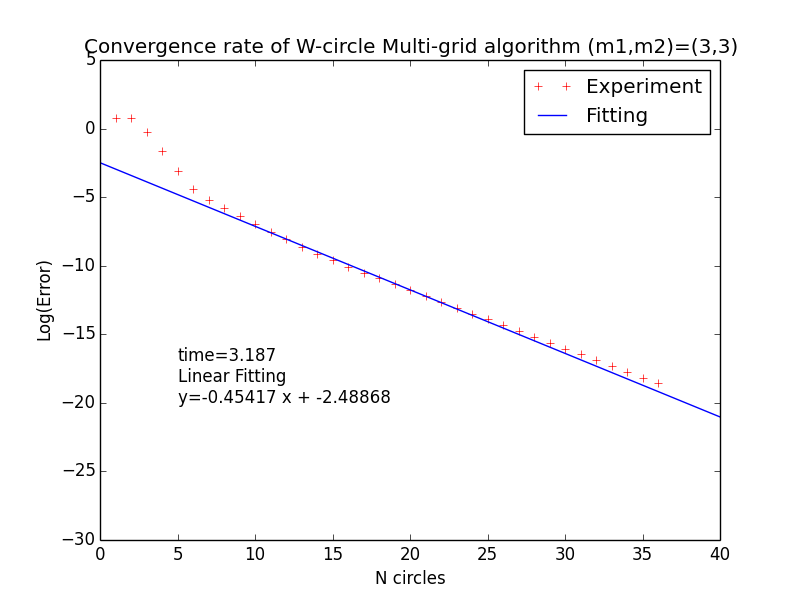
\includegraphics[width=0.4\textwidth]{W_converge_rate.png}
		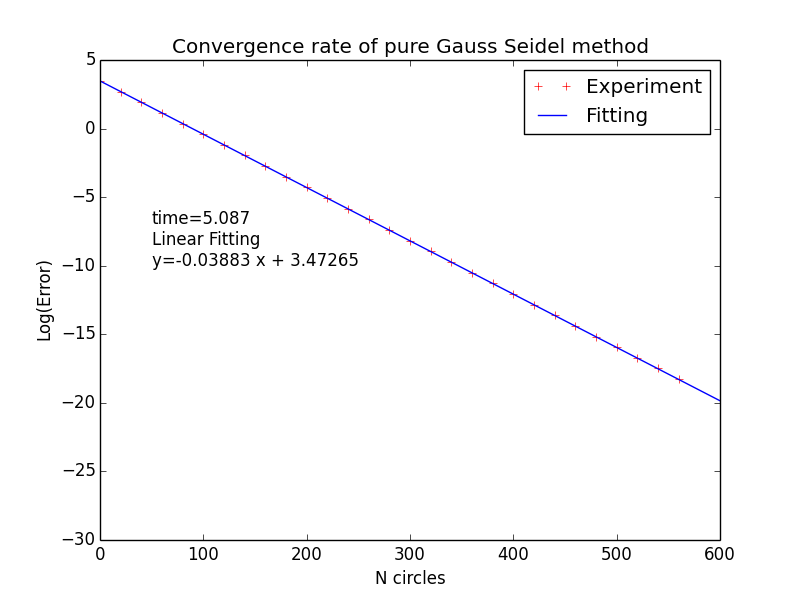
\includegraphics[width=0.4\textwidth]{GS_converge_rate.png}
		\caption{Upper LHS: V-circle error decrease exponentially, the fitting slow shows the convergence rate. Upper RHS: same figure for W-circle. Lower: Pure Gauss Seidel method (6 steps per circle).}
		\label{fig4}
	\end{center}
\end{figure}

\begin{figure}[h!]
	\begin{center}
		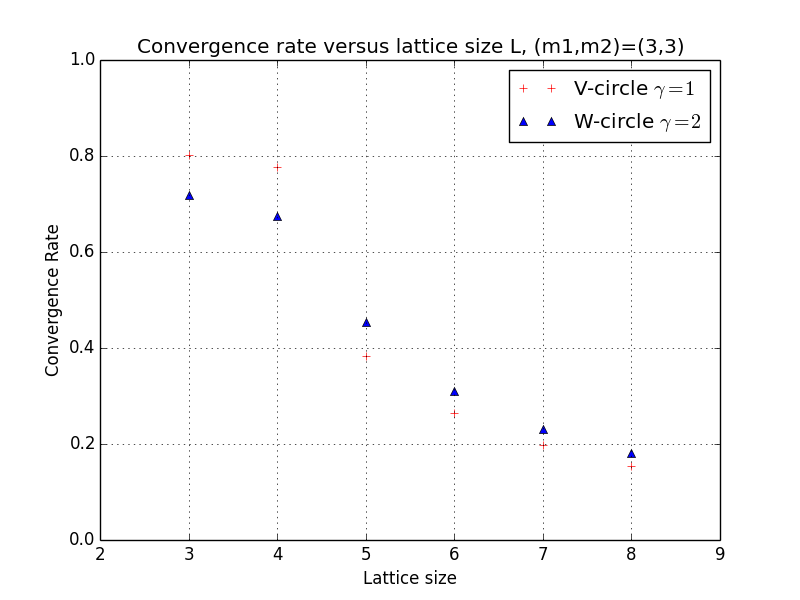
\includegraphics[width=0.4\textwidth]{rate_size.png}
		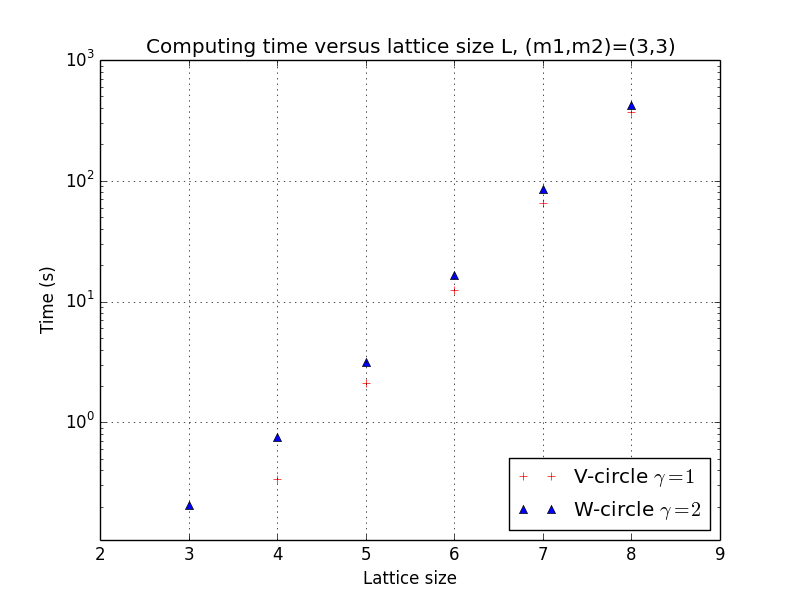
\includegraphics[width=0.4\textwidth]{time_size.png}
		\caption{LHS: Convergence rate versus lattice size $L$. RHS: Computing Time versus lattice size. Note that grid number $N=2^L$ and step size $h=\frac{1}{N}$}
		\label{fig5}
	\end{center}
\end{figure}



\subsubsection{Optimal parameter $(m_1,m_2,\gamma)$}
Table.1 shows the comparison of computing time and convergence rate using V-circle and W-circle with different pre- and post- smoothing steps. First, the more steps in total, the more time consuming during the process. Second, post-smoothing play an more important role in convergence rate. Actually, from the data I may conclude that pre-smoothing is totally redundant. V-circle $(m_1,m_2)=(0,3)$ performs as good as W-circle, but faster in a factor of almost two. Therefore, in the particular problem, I would recommend using V-circle with $(m_1,m_2)=(0,3)$.

\begin{table}[b!]
	\begin{center}
		\begin{tabular}{c|c|c|c|c|c|c}
			\hline
			V-circle$(m_1,m_2)$ & $(3,1)$& $(3,2)$& $(3,3)$ & $(2,3)$ & $(1,3)$&$(0,3)$ \\ 
			\hline
			Eclipse Time $(s)$ & $ 2.018$&$1.990$&$2.212$ &$1.603$&$1.151$&$0.701$ \\
			\hline
			Convergence Rate (slope) & $0.305$& $0.356$& $0.384$& $0.444$& $0.571$&$0.774$\\
			\hline
			\hline
			W-circle$(m_1,m_2)$ & $(3,1)$& $(3,2)$& $(3,3)$ & $(2,3)$ & $(1,3)$&$(0,3)$ \\ 
			\hline
			Eclipse Time $(s)$ & $ 2.624$&$2.967$&$3.282$ &$2.226$&$1.896$&$1.2696$ \\
			\hline
			Convergence Rate (slope) & $0.357$& $407$& $0.454$& $0.618$& $0.611$&$0.774$\\
			\hline
		\end{tabular}
	\end{center}
	\caption{Table of eclipse time and convergence rate in each method by difference pre- and post- smoothing iteration.}
\end{table}

\subsubsection{Overrelaxation parameter $\omega$}
From the previous exercise, the optimal relaxation parameter in 25-by-25 grid probem is $\omega_{opt}=1.76908771664$. At the begining, I would expect a better performance with $\omega_{opt}$ due to the same effect in the previous lessen. However, the results shows that the larger the $\omega$ is, the slower of convergence rate would be. The reason might be the correction term using prolongation from lower level as right hand side of equation. Therefore, full correction is more preferred than partially correction since these correction are precise value in higher order compare to pure Gauss Seidel method. That's why in multi-grid method $\omega=1$is preferred rather than $\omega_{opt}$.

\begin{table}[b!]
	\begin{center}
		\begin{tabular}{c|c|c|c|c}
			\hline
			V-circle  $(m_1,m_2)=(0,3)$& $\omega=1.$&$\omega=1.2$& $\omega=1.5$ & $\omega=\omega_{opt}$ \\ 
			\hline
			Eclipse Time $(s)$ & $ 0.756$&$0.707$&$0.795$ &$6.281$\\
			\hline
			Convergence Rate (slope) & $0.774$& $0.757$& $0.786$& $0.099$\\
			\hline
		\end{tabular}
	\end{center}
	\caption{Table of eclipse time and convergence rate in each method by different relaxation parameter $\omega$, where $\omega_{opt}=1.76908771664$ and $(m_1,m_2)=(0,3)$.}
\end{table}


\subsubsection{Nine-point restriction and prolongation}

Table.3 shows the effect of restriction and prolongation method. In every aspects, piecewise-linear method performs much better than nine-point does. 

\begin{table}[b!]
	\begin{center}
		\begin{tabular}{c|c|c}
			\hline
			V-circle$(m_1,m_2)=(3,3)$ &nine-point& piecewise-linear \\ 
			\hline
			Eclipse Time $(s)$ &$3.425$&$2.276$ \\
			\hline
			Convergence Rate (slope) & $0.286$& $0.384$\\
			\hline
			\hline
			W-circle$(m_1,m_2)=(3,3)$ &nine-point& piecewise-linear \\ 
			\hline
			Eclipse Time $(s)$ & $4.635$&$3.249$ \\
			\hline
			Convergence Rate (slope) & $0.31$& $0.454$\\
			\hline
		\end{tabular}
	\end{center}
	\caption{Table of eclipse time and convergence rate in V-circle and W-circle using nine-point and piecewise-linear restricetion and prolongation. 25-by-25 mesh grid are applied in this experiment}
\end{table}



\end{document}



\begin{figure}[h!]
	\begin{center}
		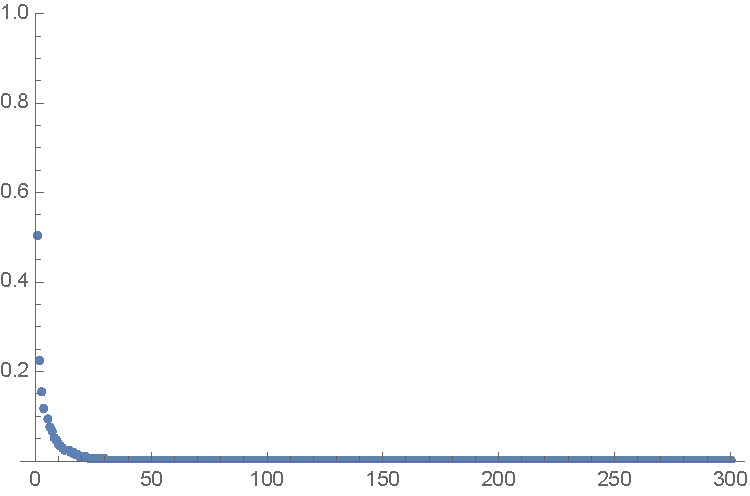
\includegraphics[width=0.4\textwidth]{a_09.pdf}
		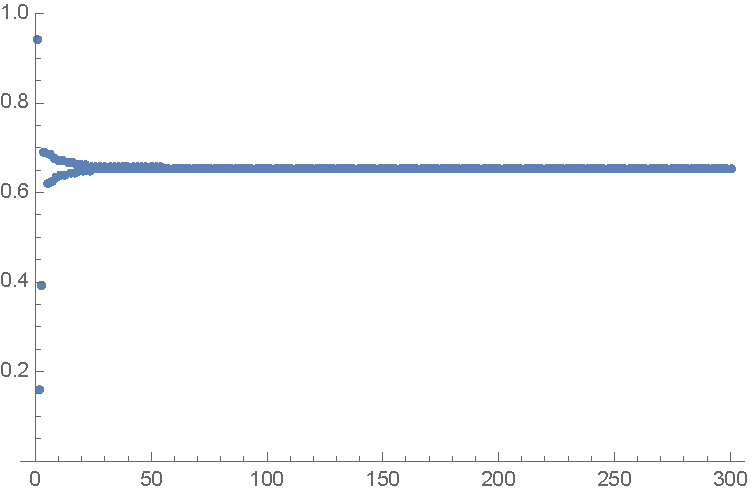
\includegraphics[width=0.4\textwidth]{a_29.pdf}
		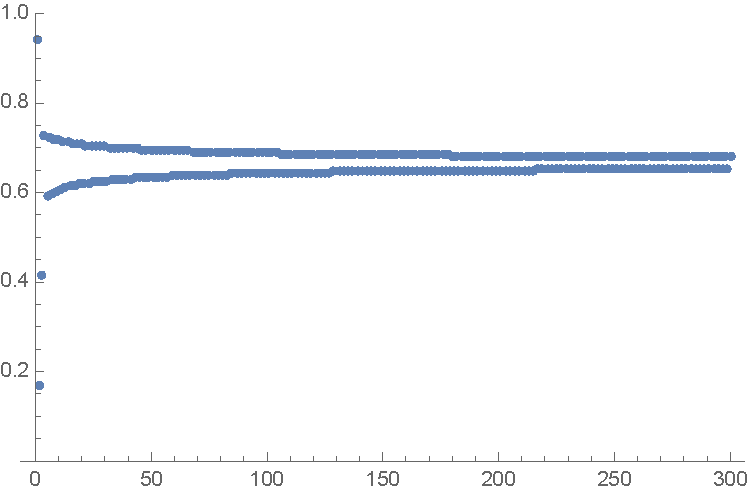
\includegraphics[width=0.4\textwidth]{a_30.pdf}
		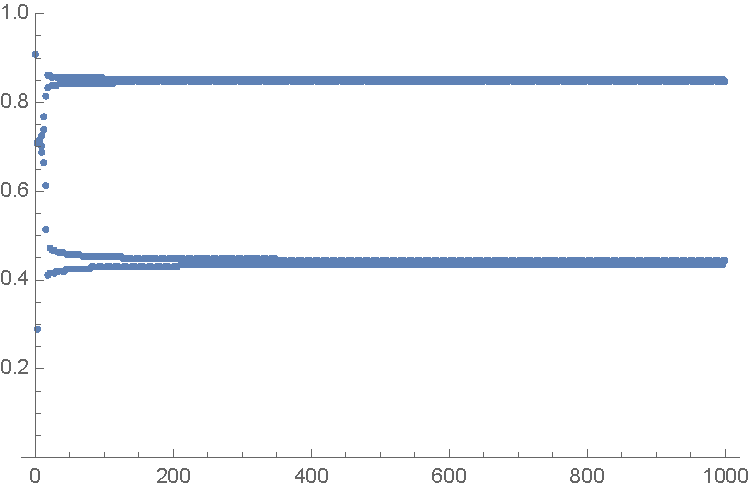
\includegraphics[width=0.4\textwidth]{a_3449.pdf}
		\caption{logistic map. Upper, left a=0.99, right a=2.9. Lower, left a=3.0, right a=3.4494.}
	\end{center}
\end{figure}

\begin{figure}[b!]
	\begin{center}
		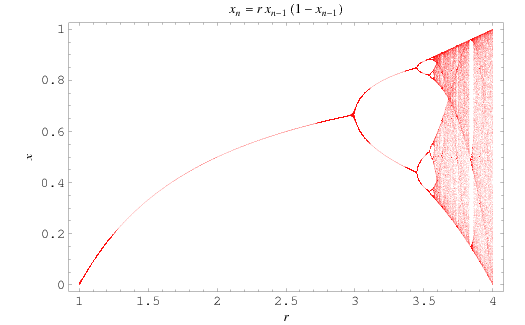
\includegraphics[width=0.8\textwidth]{logistic_map.png}
		\caption{bifurcation diagram of the logistic map. Pic. from Mahtworld}
		\label{fig1}
	\end{center}
\end{figure}


\begin{table}[h!]
	\begin{tabular}{c|lr}
		\hline
		A & $Table$ & Is\\ 
		Messy & To & Write\\
		\hline
	\end{tabular}
\end{table}


\begin{table}[h]
	\begin{center}
		\begin{tabular}{c|c}
			\hline
			period & bifurcation point a\\ 
			\hline
			2 & $0.7199616841972$ \\
			4 & $0.8332663532346$\\
			8 & $0.8591690091416$\\
			16& $0.8640801075000$*\\
			\hline
		\end{tabular}
	\end{center}
	\caption{Numerical approach to recursion sin function. First three are searching by bisection method, $\epsilon<10^{-10}$. *Last one is using step-in method, accuracy$\epsilon<10^{-5}$, although steps are much smaller than that.}
\end{table}

\begin{eqnarray}
G&&=6.67\times 10^{11} m^3 kg^{-1} s^{-2}\nonumber\\
M_{sun}&&=1.988\times 10^{30} kg\nonumber\\
c&&=3.0\times 10^8 ms^{-1}\nonumber\\
R_{orbit}&&=46\times 10^9 m\nonumber\\
v&&=58.98\times 10^3 ms^{-1}\nonumber\\
T_{period}&&=87.968 days
\end{eqnarray}